% !TEX root = ../main.tex

% Gaussian process regression section

\section{Gaussian process regression} \label{section:GPs}


Consider a sequence of random variables $X = (X_t)_{t \in \calT}$ endowed with covariates in the space $\calT$ and consider a finite subset $X_T$, $T \subset \calT$ of them. Suppose we are interested in studying $X_{t^{*}}$ for $t^{*} \notin T$, given $X_T$. A natural estimator would be $\bbE [X_{t^{*}} \, | \, \sigma X_T ]$, which of course depends on the distributional and dependence structures of the process $X$. If $X$ is a Gaussian process, which we define below, this expression can be easily computed and the methodology just discusses is called Gaussian process regression. This method has gained popularity in the last years as a reliable way of modelling complex phenomena, such as computer experiments \cite{SacksEtAl:1989:CompExp} and disease spreading modeling \cite{PokharelDeardon:2016:GPInfectDisease}, and for doing Bayesian optimization \cite{Frazier:2018:BayesOptTutorial} and statistical emulation \cite{WoodsEtAl:2017:ACEAlgorithm}.



\begin{definition}[Gaussian process] \label{def:GP}
	A stochastic process $X = (X_t)_{t \in \calT}$ is said to be a Gaussian process (GP) if, for any finite subset $T \subset \calT$, $X_T$ follows a Normal distribution. 
\end{definition}


\textbf{Remark.} A Gaussian process is entirely determined by its mean $m$ and covariance $\kappa$ functions. Formally, $m: t \mapsto \bbE[X_t]$ and $\kappa: (t, t') \mapsto \Cov(X_t, X_{t'})$ and we write $X \sim \GP (m, \kappa)$. Commonly, $m$ is assumed to be zero and $\kappa$ is chosen from some parametric family of functions, many of which have been thoroughly studied in the literature \cite[see][Ch.~4]{RasmussenWilliams:2006}. Unless otherwise stated, we use a standard squared exponential covariance function,
\begin{equation} \label{eq:sq_exp_cov}
	\kappa(t, t') = \kappa(|t-t'|) = \mathrm{exp} \left\{ -\frac{1}{2} |t-t'|^2 \right\}.
\end{equation}



In practice, GP regression commonly arises when studying functions which are computationally expensive to evaluate. The general idea is to assume that the function of interest $f$ is a GP and use a sample of values of $f$ to estimate the function in unobserved values of the domain. Formally, consider a function $f: \calT \to \bbR$ and denote $X_t := f(t)$ for all $t \in \calT$. We assume that $X = (X_t) \sim \GP (m, \kappa)$. Usually, $\calT$ will be a subset of $\bbR^n$, $m = 0$ and we will have access to observations $(X_t, t)_{t \in T}$, where $T$ is a finite subset of $\calT$. If this is the case,
\begin{equation} \label{eq:GP_noise_free}
	X_T \equdist \calN (0, K(T, T)),
\end{equation}
where $K$ is a $|T| \times |T|$ matrix with entries $K_{ij} = \kappa(t_i, t_j)$. If we want to predict the value of the function $f(t^{*})$, we again use the fact that
\begin{equation*}
	\begin{pmatrix} X_T \\ X_{t^{*}} \end{pmatrix} \equdist \calN \left( 0, \begin{pmatrix} K(T, T) & K(T, t^{*}) \\ K(t^{*}, T) & \kappa(t^{*}, t^{*}) \end{pmatrix} \right),
\end{equation*}
from where, using basic properties of the Normal distribution,
\begin{equation} \label{eq:GPupdate}
	\bbP [X_{t^{*}} \,| \, \sigma X_T ] \equdist \calN \left( K(t^{*}, T) K(T, T)^{-1} X_T, \, \kappa(t^{*}, t^{*}) K(t^{*}, T) K(T, T)^{-1} K(T, t^{*})  \right).
\end{equation}
Equation (\ref{eq:GPupdate}) gives us not only the conditional expectation discussed earlier, but the whole conditional distribution: $\bbP [X_{t^{*}} \,| \, \sigma X_T ]$ is a Normally-distributed random variable. Commonly, the conditional mean in Equation (\ref{eq:GPupdate}) is used as a point estimate $\tilde{f}$ of $f$:
\begin{equation} \label{eq:GP_posteriormean}
	\tilde{f} (t^{*}) = \bbE [ X_{t^{*}} \, | \, \sigma X_T ] = K(t^{*}, T) K(T, T)^{-1} X_T.
\end{equation}
The estimated variance can be used to e.g. compute (conditional) confidence bands. Also, observe that we could have well chosen $t^{*}$ to have more than one component if we were interested in values of $f$ only at specific points in the covariate space. The advantage of Equation (\ref{eq:GP_posteriormean}) is that it provides point estimates for \textit{any} point in $\calT$. Figure \ref{fig:GP1} showcases this process. \\




\begin{figure}[h]
	\centering
	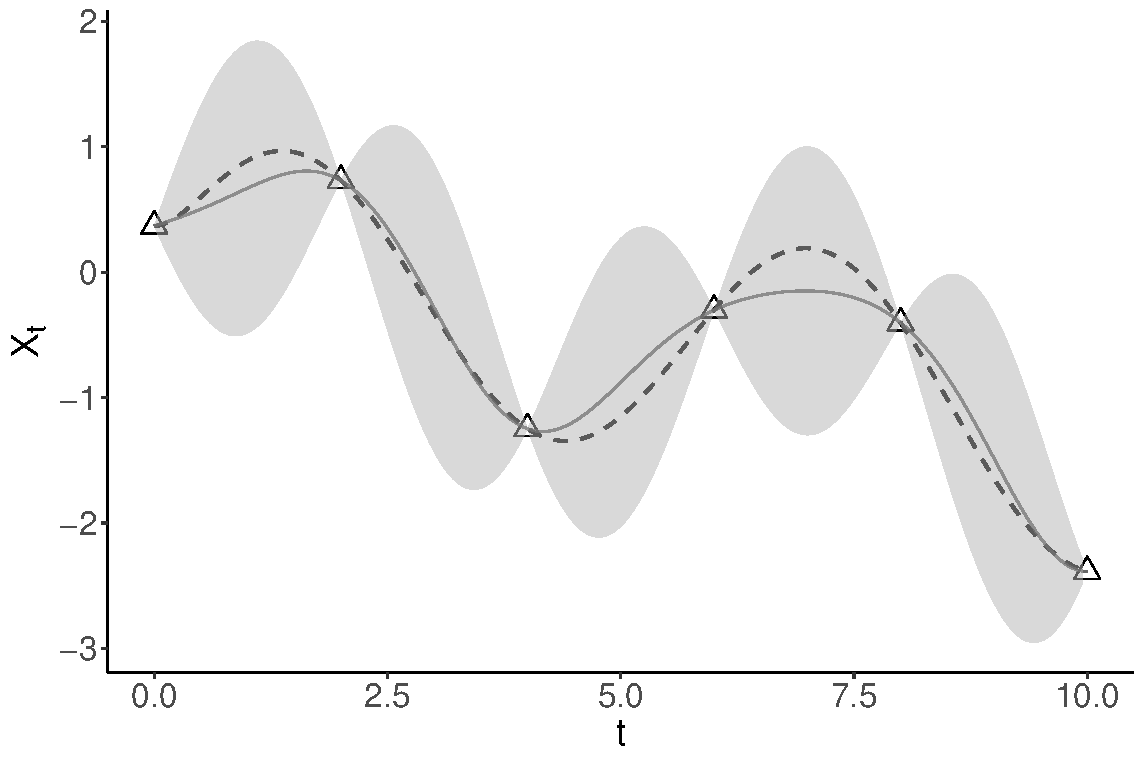
\includegraphics[scale=0.5]{GP1.pdf}
	\caption{Gaussian process regression used to estimate a function $f = X_t$ (shown in dotted grey lines). The prediction is based on the conditional mean of a noise-free GP with squared exponential function, which is shown in a line and was fitted based on 6 observations of $f$ (the triangle shapes). 95\% confidence bands computed using the conditional variance are also shown.}
	\label{fig:GP1}
\end{figure}



It is easy to extend this idea for cases in which, rather than having access to exact values of the function $f$, only estimates with some noise are available. This is the case, for example, when $f$ is simply impossible to evaluate, but can be reliably estimated via Monte Carlo methods---e.g. when $f$ is an expected loss over a high-dimensional parameter space. In these situations an additive noise term $\sigma^2$ is commonly added to the covariance function $\kappa$ for observations with the same covariates: $\kappa_{\sigma} (t, t') = \kappa(t, t') + \sigma^2 \, \indicator (t = t')$, where $\kappa$ is a regular noise-free covariance function. For any finite subset $T \subset \calT$, this can be represented as
\begin{equation*}
	K_{\sigma} (X_T, X_T) = K(X_T, X_T) + \sigma^2 \, I_{|T|},
\end{equation*}
so that
\begin{equation} \label{eq:GP_noise}
	X_T \equdist \calN \left( 0, \, K(T, T) + \sigma^2 \, I_{|T|} \right).
\end{equation}
The resulting conditional distribution for a new covariate value $t^{*}$ given $T$ is
\begin{equation*}
 \bbP [X_{t^{*}} \,| \, \sigma X_T ] \equdist \calN \left( K(t^{*}, T) \left( K(T, T) + \sigma^2 \, I_{|T|} \right)^{-1} X_T, \, \kappa(t^{*}, t^{*}) K(t^{*}, T) \left( K(T, T) + \sigma^2 \, I_{|T|} \right)^{-1} K(T, t^{*})  \right).
\end{equation*}



\subsection{Exchangeability of Gaussian processes}


We now study exchangeability in the context of Gaussian process regression. Let $X = (X_t)_{t \in \calT} \sim \GP (0, \kappa)$. The process $X$ is said to be noise-free if Equation (\ref{eq:GP_noise_free}) holds and $\sigma$-noisy if Equation (\ref{eq:GP_noise}) holds for any finite subset $T \subset \calT$. We assume that $\kappa$ is given by Equation (\ref{eq:sq_exp_cov}), possibly with a modification to account for noisy observations if necessary, and that $\calT \subset \bbR$.



\begin{proposition} \label{prop:exchangeability}
	Let $X = (X_t)_{t \in \calT} \sim \GP (0, \kappa)$. Then $X$ is not exchangeable.
\end{proposition}

\textbf{Proof. \hspace{0.05cm}} Conceptually this is trivially true, and is due to the fact that the covariance function $\kappa$---which completely determines the process---is sensible to the distance between covariates. The order of the covariates matters, and so the sequence cannot be exchangeable. Formally, let $T = \{ t_1, t_2, t_3 \}$ with $t_2 = t_1 + 1, t_3 = t_1 + 2$ and $\pi$ be a permutation of $T$ such that $\pi(t_1) = t_2$,  $\pi(t_2) = t_1$, and $\pi(t_3) = t_3$. Then $X_T = \calN (0, K(T, T))$ and $X_{\pi T} = \calN(0, K(\pi T, \pi T)$. If $X$ were exchangeble, then $X_T \equdist X_{\pi T}$, and particularly $\kappa(t_1, t_3) = \kappa(t_2, t_3)$, which is clearly not the case because $\kappa(t_1, t_3) = e^{-1}$ but $\kappa(t_2, t_3) = e^{-1/2}$, regardless of whether the process is noisy or not.

\qed

\vskip 0.2cm

One may argue that this result is more due to the specific covariance function we chose rather than some underlying principle, but this is not so: the covariance function \textit{has} to be sensible to some notion of distance between covariates because we assume that close covariates will yield somewhat similar values of the function. The prediction of the process at $t^{*}$ includes information from all observations in $T$, but naturally those values in $T$ closer to $t^{*}$ will have a greater weight on the estimate $\bbE [X_{t^{*}} \, | \, \sigma X_T ]$. \\


The exchangeability requirement in Proposition \ref{prop:exchangeability} can be weakened to yield positive results, as we now show.

%but first we follow \cite{CampbellEtAl:2019:LocalExch} and introduce the following notation. Let $X = (X_t)_{t \in \calT}$ be a noisy Gaussian process with $\calT = \bbR$. If it is possible to obtain multiple observations at a single value, then it makes sense to modify $\calT$ by $\tilde{\calT} = \bbR \times \bbN$, where the first entry would denote the location of the observation and the second one the number of observation. So $\tilde{t} = (0.56, 2)$ would refer to the second observation at the value $t = 0.56$. In such a scenario we use both $\calT$ and $\tilde{\calT}$ interchangeably depending on the context; particularly when dealing with local exchangeability, using $\tilde{\calT}$ is more convenient. \\


\begin{proposition} \label{prop:GP_partial_exch}
	Let $X = (X_t)_{t \in \calT} \sim \GP (0, \kappa)$ be a $\sigma$-noisy Gaussian process. Then $X$ is partially exchangeable.
\end{proposition}

\textbf{Proof. \hspace{0.05cm}} The idea is to group the process into sequences with the same covariate value and prove that each of those is exchangeable. Formally, let $X_{t_0} = (X_{t_0, \, n})_{n=1}^{\infty}$ be the $t_0$-class of $X$ for each (distinct) $t_0 \in \calT$. Let $N = \{n_1, ..., n_r \}$ and $\pi$ a permutation of $N$. The key observation here is that $\kappa(t_0, t_0) = 1$, and so
\begin{equation} \label{eq:GP_partial_exchangeability}
	X_{t_0 \, N} \equdist \calN (0, (1+\sigma^2) I_r) \equdist X_{t_0 \, \pi N}.
\end{equation}
This proves that each $t_0$-class is exchangeable, and thus the whole process is partially exchangeable.

\qed

\vskip 0.2cm

A good question is whether a noise-free GP is partially exchangeable. We argue to the contrary, asserting---as in the previous section---that partial exchangeability is defined with replicates in mind. If a function can be precisely estimated (even if expensively so) at any given value $t$, it makes no sense to obtain replicates: there is no within-covariate variability. 
\\

%Indeed, if one attempts to replicate the previous proof then Equation (\ref{eq:GP_partial_exchangeability}) still holds, albeit with degenerate Normals that have zero variance. \\



In preparation for the main local-exchangeability results for GP regression, we state a sufficiency condition for determining local exchangeability of a sequence. For a proof, see \cite[][Proposition 3]{CampbellEtAl:2019:LocalExch}.

\begin{proposition} \label{prop:sufficient_local_exchangeability}
	Consider a process $(X_t)_{t \in \calT}$ and suppose there exists a $\sigma$-algebra $\calG$ such that, for any finite subset $T \subset \calT$ of covariates, the components of $X_T$ are conditionally independent given $\calG$. Let $G_t = \bbP [X_t \, | \, \calG ]$. Then $X$ is $f$-locally exchangeable if, for all pairs $t, t' \in \calT$,
	\begin{equation} \label{eq:sufficient_local_exchangeability}
		\bbE[d_{\mathrm{TV}} (G_t , G_{t'} ) ] \leq f(d(t, t')).
	\end{equation}
\end{proposition}

Now we assert that $\sigma$-noisy GPs are $f$-locally exchangeable, where $f$ is inversely proportional to the noise factor $\sigma$. 

\begin{proposition} \label{prop:GP_local_exchangeability}
	Let $f(x) = x / \pi \sigma$ and $X = (X_t)_{t \in \bbR} \sim \GP (0, \kappa)$ be a $\sigma$-noisy Gaussian process in $\bbR$, which we furthermore endow with the metric  $d(t, t') = |t-t'|$. Then $X$ is $f$-locally exchangeable.
\end{proposition}



\textbf{Proof. \hspace{0.05cm}} We prove that the requirements of Proposition \ref{prop:sufficient_local_exchangeability} are met. First observe that
\begin{equation*}
	\kappa(t, t') = \mathrm{exp} \left\{ -\frac{1}{2} |t - t'|^2 \right\} \geq 1 - \frac{1}{2} |t-t'|^2 = 1 - \frac{1}{2} d(t, t')^2,
\end{equation*}
which can be proved via the Taylor series expansion of $\mathrm{exp} \left\{ -\frac{1}{2} y^2 \right\}$. This can also be rewritten as
\begin{equation} \label{eq:kappa_bound}
	1 - \kappa(t, t') \leq \frac{1}{2} d(t, t')^2.
\end{equation}
Now let $T \subset \bbR$ be a finite subset of covariates of size $n$. Denoting $K(T, T) = K$, by Equation (\ref{eq:GP_noise}) we have that $X_T \equdist \calN (0, K + \sigma^2 I_n )$. Now let $Y_T \equdist \calN(0, K)$ and observe that
\begin{equation}
	\bbP [X_T \, | \, \sigma Y_T ] \equdist \calN(Y_T, \sigma^2 I_n).
\end{equation}
Thus, for every $t \in T$ the conditional distribution of $X_t$ given $Y_t$ is $G_t \equdist \calN (Y_t, \sigma^2)$. We need only prove that $\bbE[d_{\mathrm{TV}} (G_t , G_{t'} ) ] \leq f(d(t, t'))$. But, as per \cite[][p.~15]{CampbellEtAl:2019:LocalExch}, the total variation between two Normal distributions can be expressed in terms of the cumulative distribution function $\Phi$ of a standard Normal distribution, and so
\begin{align}
	d_{\mathrm{TV}} (G_t , G_{t'} )  &= d_{\mathrm{TV}} (\calN (Y_t, \sigma^2) , \calN (Y_{t'}, \sigma^2) )   \nonumber \\
		&= \Phi \left( \frac{|Y_t - Y_{t'} |}{2 \sigma} \right) - \Phi \left( -\frac{|Y_t - Y_{t'} |}{2 \sigma} \right) \nonumber \\
		&\leq \frac{|Y_t - Y_{t'} |/2\sigma + |Y_t - Y_{t'} |/2\sigma}{\sqrt{2\pi}} && \text{(by Lemma \ref{lemma:lipschitz})} \nonumber \\
		&= \frac{|Y_t - Y_{t'}|}{\sqrt{2 \pi \sigma^2}}. \label{eq:TV_GP}
\end{align}
Now, observe that $\kappa(t, t) = 1$ for all $t \in \bbR$, and so $Y_t, Y_{t'} \equdist \calN(0, 1)$ are Normal (and jointly Normal too by construction). Furthermore, $\mathrm{cov}(Y_t, Y_{t'}) = \kappa(t, t')$, and so by Lemma \ref{lemma:halfnormal}
\begin{equation*}
	\bbE |Y_t - Y_{t'}| = \sqrt{\frac{4}{\pi}(1 - \kappa(t, t'))}.
\end{equation*}
Substituting in Equation (\ref{eq:TV_GP}) we deduce
\begin{equation} \label{eq:TV_GP_2}
	\bbE [d_{\mathrm{TV}} (G_t , G_{t'} )] \leq \sqrt{\frac{2}{\pi^2 \sigma^2}(1 - \kappa(t, t'))}.
\end{equation}
Using $\kappa$'s lower bound (Equation \ref{eq:kappa_bound}) we finally get that, for all $t, t'$,
\begin{equation}
	\bbE [d_{\mathrm{TV}} (G_t , G_{t'} )] \leq \sqrt{\frac{1}{\pi^2 \sigma^2}d(t, t')^2} = \frac{d(t, t')}{\pi \sigma}.
\end{equation}
The result follows from Proposition \ref{prop:sufficient_local_exchangeability} with $f(x) = \frac{x}{\pi \sigma}$.

\qed


\vskip 0.25cm

It is not immediatly clear from the proof whether this result holds for noise-free GPs. The argument essentially splits the variability in each observation into the variability within ($\sigma$) and between ($K$) covariates, and takes advantage of the fact that the within-covariate variability does not depend on the actual value of the covariate. But if no replicates are available, the argument no longer works and the function $f$ is not even defined, for we would have $\sigma = 0$. \\

On the other hand, recalling the definition of local exchangeability (Definition \ref{def:local_exchangeability}), it is intuitively clear that noise-free GPs should be locally exchangeable. It turns out that it is possible to modify the previous argument to get a positive result for noise-free GPs. We state the result, although the proof is left as an exercise.



\begin{proposition} \label{prop:GP_NF_local_exchangeable}
	Let $f(x) = (2/\pi) x$ and $X = (X_t)_{t \in \bbR} \sim \GP (0, \kappa)$ be a noise-free Gaussian process in $\bbR$, which we furthermore endow with the metric  $d(t, t') = |t-t'|$. Then $X$ is $f$-locally exchangeable.
\end{proposition}

\textbf{Proof. \hspace{0.05cm}} See Exercise \ref{ex:GP_NF_local_exchangeable}. \\



We now assert the corresponding result for regression exchangeability.


\begin{proposition} \label{prop:GP_reg_exch}
	Let $X = (X_t)_{t \in \calT} \sim \GP (0, \kappa)$ be a Gaussian process. Then $X$ is regression exchangeable.
\end{proposition}



\textbf{Proof. \hspace{0.05cm}} Let $T_1, T_2 \subset \calT$ be finite and first assume $X$ is noise-free.
\begin{enumerate}
	\item For Condition \ref{cond:reg_exch_1}, suppose $T_1 \subset T_2$.  We know $X_{T_2} \equdist \calN (0, K(T_2, T_2))$, and basic properties of the Normal distribution tell us that the distribution of $X_{T_1}$ is the same as that of $X_{T_2}$ but removing the coordinates in $T_2 \setminus T_1$.
	\item For Condition \ref{cond:reg_exch_2}, suppose $T_1 = T_2$. Because the process is noise-free, this means that $X_{T_1} = X_{T_2}$ exactly, and so $X_{T_1} \equdist X_{T_2}$.
\end{enumerate}
The case for $\sigma$-noisy GPs follows from simple modifications to the previous arguments. Namely, $X_{T_2} \equdist \calN( 0, K(T_2, T_2) + \sigma I)$ and the distribution of $X_{T_1}$ is again obtained by coordinate deletion for Condition \ref{cond:reg_exch_1}. For Condition \ref{cond:reg_exch_2} the only caveat is that $X_{T_1}$ and $X_{T_2}$ may contain different replicates, but they do so at the same covariates, and so both follow the same $\calN (0, K(T, T) + \sigma I)$ distribution, with common $T = T_1 = T_2$.

\qed






% ...